\documentclass[20pt,margin=2.2cm,innermargin=-4.5in,blockverticalspace=-0.25in]{tikzposter}

\geometry{paperwidth=80cm,paperheight=120cm} %A0
% \geometry{paperheight=33.11in,paperwidth=23.4in} %A1
\usepackage[utf8]{inputenc}
\usepackage[spanish]{babel}
\usepackage{amsmath}
\usepackage{amsfonts}
\usepackage{amsthm}
\usepackage{amssymb}
\usepackage{mathrsfs}
\usepackage{graphicx}
\usepackage{lipsum}
\usepackage[export]{adjustbox}
\usepackage{enumitem}
\usepackage[backend=biber,style=numeric]{biblatex}
\usepackage{ubtheme}
\makeatletter
\setlength{\TP@visibletextwidth}{75cm}
\setlength{ \TP@visibletextheight}{45in}
\makeatother
\usepackage{mwe} % for placeholder images
\usepackage{bm}
\usepackage{bbm}
\definecolor{bristolred}{HTML}{B01C2E}
\addbibresource{refs.bib}

% set theme parameters
\tikzposterlatexaffectionproofoff
\usetheme{UBTheme}
\usecolorstyle{UBStyle}
\useinnerblockstyle{Heldert}
\def \SL{SL_2(\mathbb{Z})}
\def\H{{ \!\! \rm \ I\!H}}
\newcommand{\set}[1]{ \left\{ #1 \right\} }

\makeatletter
\newcounter{tablecounter}
\newenvironment{tikztable}[1][]{
  \def \rememberparameter{#1}
  \vspace{10pt}
  \refstepcounter{tablecounter}
  \begin{center}
  }{
    \ifx\rememberparameter\@empty
    \else
    \\[10pt]
    {\small Tab.~\thetablecounter: \rememberparameter}
    \fi
  \end{center}
}
\makeatother

\usepackage[scaled]{helvet}
\renewcommand\familydefault{\sfdefault} 
\renewcommand{\vec}[1]{\bm{#1}}
\newcommand{\Tr}{\text{Tr}}
\usepackage[T1]{fontenc}

\title{\parbox{0.95\linewidth}{Una antolog\'ia de la obra de Conway}}
\author{\textbf{Roger David Trujillo Ib\'a\~nez}\textsuperscript{1}}
\institute{\textsuperscript{1}Departamento de Matemáticas, Universidad Nacional de Colombia}

\titlegraphic{
\includegraphics[width=0.23\textwidth]{Imagenes/PNG_LOGOSIMBOLO_LATERAL_NEGRO-02.png}}

% begin document
\begin{document}
\maketitle
\begin{columns}
    \column{0.5}
    \block{Descripción General}{En este trabajo se calculó el género del espacio topológico que se considera al tomar las orbitas de $\H$ (plano complejo superior) bajo la acción de $$\Gamma(N)=\set{\left(\begin{smallmatrix}a&b\\c&d\end{smallmatrix}\right)\in\SL:\left(\begin{smallmatrix}a&b\\c&d\end{smallmatrix}\right)\equiv\left(\begin{smallmatrix}1&0\\0&1\end{smallmatrix}\right)}$$
    dada por 
    \begin{equation}
        \left(\begin{smallmatrix}a&b\\c&d\end{smallmatrix}\right)\tau=\frac{a\tau+b}{c\tau+d}
    \end{equation}
    Con este fin exploramos la estructura compleja del cociente para poder utilizar el teorema de Riemann-Hurwitz, y así obtener que el género del espacio $\H^*/\Gamma(N)$ (para $N\leq3$) es
    \begin{equation}
        g_N=1+\frac{N^2(N-6)}{24}\prod_{p|N}\left(1-\frac{1}{p^2}\right)
    \end{equation}
    }
    

    
    \block{El juego de la vida}{
        Conway cuenta que fueron las ideas de c\'omo los aut\'omatas podr\'ian en alg\'un momento simular cosas complejas como el cerebro humano, o incluso, podr\'ian replicarse a s\'i mismas, las que dieron inicio a su inter\'es en crear aut\'omatas. Conway empez\'o a buscar automatas universales que tuvieran reglas simples. La idea de Von Neumann era sobre una cuadr\'icula de dos dimensiones, as\'i que Conway pens\'o primero en algo m\'as simple, algo de una sola dimensi\'on, FRACTRAN fue el primer resultado.
        \vspace{7mm}
        
        \innerblock{FRACTRAN}{
            Es un lenguaje de programaci\'on cuyos programas consisten en una lista finitas de fracciones, y puede crear cualquier programa posible, por ejemplo, este es un programa que genera los n\'umeros primos en orden
            \[
                {\displaystyle \left({\frac {17}{91}},{\frac {78}{85}},{\frac {19}{51}},{\frac {23}{38}},{\frac {29}{33}},{\frac {77}{29}},{\frac {95}{23}},{\frac {77}{19}},{\frac {1}{17}},{\frac {11}{13}},{\frac {13}{11}},{\frac {15}{14}},{\frac {15}{2}},{\frac {55}{1}}\right)}.
            \]

        }

        \vspace{5mm}
        Despues de esto, Conway intent\'o jugar con aut\'omatas de una dimension, es decir aut\'omatas donde la cuadr\'icula es de solo un cuadro de ancho. Sin embargo, se le hizo muy dificil tener resultados sobre estos \cite{Roberts2015-ur}. Fue hasta que lo intent\'o con dos dimensiones cuando lleg\'o a conseguir su cometido.

        El juego de la vida se juega en un tablero dos dimensional conformado por celdas, como un tablero de Go pero infinito. El juego empieza con un estado inicial y va evolucionando conforme a las reglas. Cada celda tiene 8 celdas adyacentes a los que llamaremos vecinos, cuatro que comparten un lado y cuatro que comparten solamente un v\'ertice, es decir, dos horizontales, dos verticales, y cuatro en diagonal. Las reglas del juego son:
        \vspace{7mm}
        
        \innerblock{Reglas}{
            \begin{enumerate}
                \item \textbf{Regla de nacimiento:} Si una celda est\'a muerta en el tiempo $t$, y la celda tiene exactamente $3$ celdas vecinas que est\'an vivas, entonces la celda se convierte en una celda viva en el tiempo $t+1$.
                \item \textbf{Regla de muerte:} Si una celda viva en el tiempo $t$ tiene menos que $2$ vecinos vivos, la celda muere por soledad en el tiempo $t+1$. Si una celda viva en el tiempo $t$ tiene m\'as que $3$ vecinos vivos, la celda muere por hacinamiento en el tiempo $t+1$.
                \item \textbf{Regla de supervivencia:} Si una celda viva tiene exactamente $2$ o $3$ celdas vivas vecinas, entonces la celda sigue viva en el tiempo $t+1$.
            \end{enumerate}

        }

        \vspace{5mm}
        En la izquierda se muestra la configuraci\'on en el paso $t=0$, a la derecha en la iteraci\'on siguiente $t=1$. A esta figura se le conoce como \textit{blinker}.
        \vspace{7mm}

        \begin{minipage}[t]{\linewidth}
            \centering
            \begin{minipage}[t]{0.4\linewidth}
                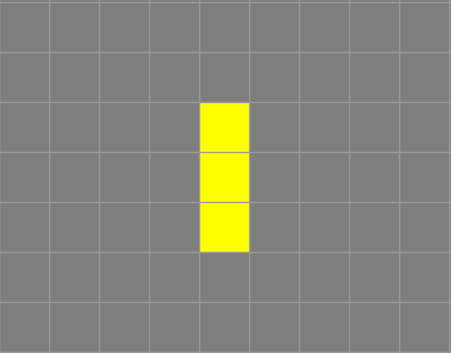
\includegraphics[width=\textwidth]{images/life-1.png}
            \end{minipage}
            \begin{minipage}[t]{0.4\linewidth}
                \setlength{\parindent}{1em}
                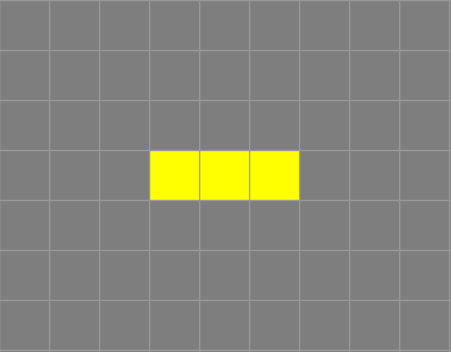
\includegraphics[width=\textwidth]{images/life-2.png}
            \end{minipage}
        \end{minipage}

        \vspace{5mm}
        En Octubre de 1970, Martin Gardner en su columna \textit{Mathematical Games} del \textit{Scientific American} \cite{Gardner1970} escribi\'o un texto titulado \textit{The fantastic combinations of John Conway's new solitaire game ``life''}. La columna, adem\'as de describir el juego propon\'ia un reto; encontrar un patr\'on inicial que al evolucionar creciera sin l\'imites, y adem\'as promet\'ia 50 USD a quien fuera el primero en encontrarla o demostrar que no existe.

        En Noviembre del a\~no en que sali\'o la columna de Gardner (1970), un equipo del MIT liderado por Bill Gosper, un matem\'atico y programador estadounidense, se gan\'o el premio propuesto en la columna al descubrir/inventar una pistola de gliders ahora conocida como la \textit{Gosper Glider gun}
        \vspace{7mm}

        \begin{minipage}[t]{\linewidth}
            \centering
            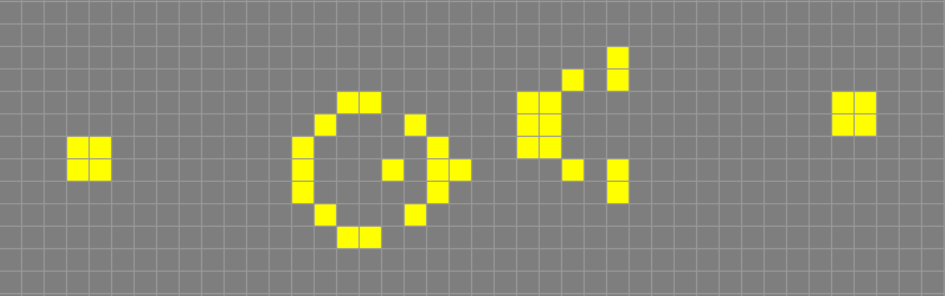
\includegraphics[width=.8\textwidth]{images/life-gosper-gun.png}
        \end{minipage}

    }
    

    
    

    \column{0.5}
    
    \block{Referencias}{
                \begin{center}
                   \mbox{}\vspace{-1\baselineskip}
    \printbibliography[heading=none] 
        \end{center}
        }

\end{columns}
\end{document}